\documentclass{beamer}
\usepackage[utf8]{inputenc}
\usepackage[francais]{babel}
\usepackage[utf8]{inputenc}  
\usepackage{listings}
\usepackage{graphicx}
\usepackage{color}
\usepackage{float}
\usepackage{algorithm}
\usepackage{algorithmic}
\usepackage{caption}

\usepackage{array}
\usepackage{colortbl}
\usepackage{amsfonts}
\usepackage{geometry}
\usepackage{setspace}
\usepackage{hyperref}
\usepackage{subcaption}
\usepackage{listings}
\usetheme{Warsaw}


\PassOptionsToPackage{demo}{graphicx}




\author{Adrien Guilbaud}
\title{Simulation numérique directe de la combustion turbulente}
%\subtitle{Presentation Subtile}
%\institute{Université de Bordeaux}
%\date{\today}


%\titlegraphic{
\includegraphics[width=2cm]{figures/logo_fac.jpg}\hspace*{4.75cm}~%
%   
\includegraphics[width=2cm]{figures/logo_cerfacs.eps}
%}


\begin{document}
 

\begin{frame}
    \parbox[c]{-50cm}{\centering%
      
\includegraphics[width=2cm]{figures/logo_fac.jpg}%
    }%
    \parbox[c]{19.5cm}{\centering%
      
\includegraphics[width=2cm]{figures/logo_cerfacs.eps}
    }%
\maketitle

\centering
\footnotesize
\begin{tabular}{cc}
  Maître de stage & Enseignant responsable \\
  Mme.~Isabelle \textsc{D'ast} &   Mr.~Samuel \textsc{Thibault} \\
  \end{tabular}
\end{frame}

%
% INTRO
%

\section{Introduction}
\subsection{Présentation du Cerfacs}
\begin{frame}
  \begin{itemize}
  \item Centre Européen de Recherche et de Formation Avancée en Calcul Scientifique
  \item Airbus Group, Cnes, EDF, Météo France, Onera, Safran et Total
  
    \begin{block}{Titre}
      Résolution de problèmes scientifiques par la résolution numérique
    \end{block}
  \end{itemize}


  \begin{itemize}
  \item climat
  \item aéronautique
  \item spatial
  \item environnement
  \end{itemize}
\end{frame}

%https://en.wikipedia.org/wiki/Discretization_of_Navier%E2%80%93Stokes_equations
\subsection{Mécanique des fluides numérique}
\begin{frame}
  \begin{block}{Mécanique des fluides}
    Etude du comportement des fluides lorsqu'ils sont en mouvement
  \end{block}
  
  \begin{itemize}
  \item Résolution des équations de Navier-Stokes
  \item Discrétisation de l'espace
  \end{itemize}
\end{frame}


\subsection{Simulation de la turbulence}
\begin{frame}
  \begin{itemize}
  \item \textit{DNS}: Direct Numerical Simulation
  \item \textit{LES}: Large Eddy Simulation
  \end{itemize}

  \begin{figure}[ht]
  \centering
  \begin{subfigure}[b]{0.5\textwidth}
    \centering
    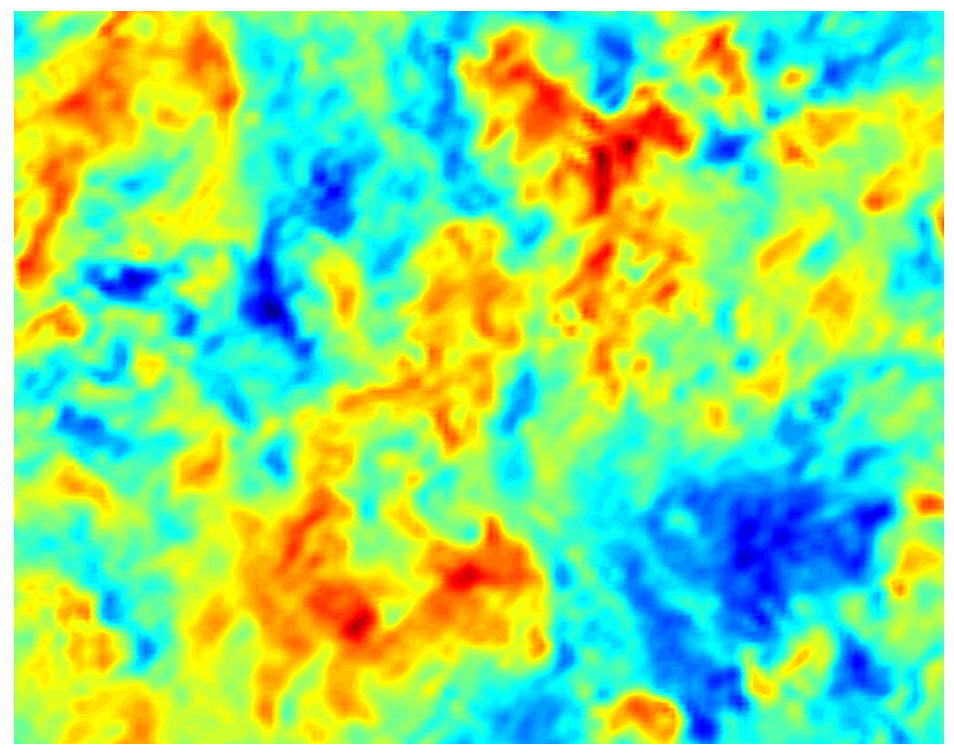
\includegraphics[scale=0.25]{figures/DNS_Velocity_Field.png}
    \caption{\label{fig:dns} Simulation des turbulences (DNS)}
  \end{subfigure}%
  ~
  \begin{subfigure}[b]{0.5\textwidth}
    \centering
    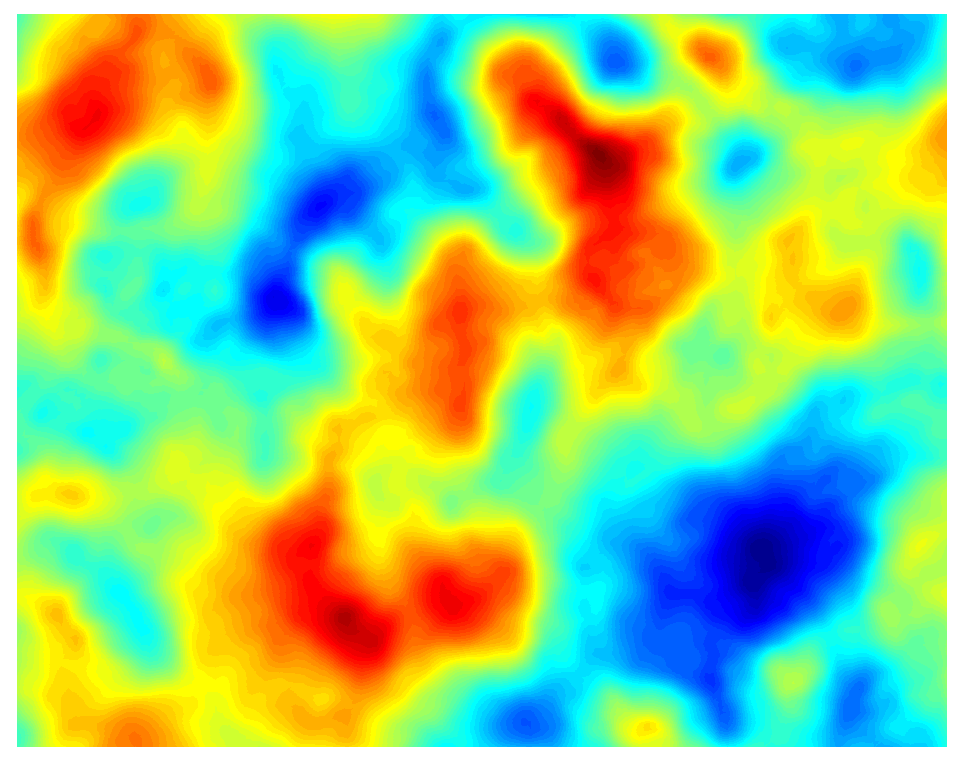
\includegraphics[scale=0.25]{figures/DNS_Filtered_Velocity_Field_Large.png}
    \caption{\label{fig:les} Simulation des grandes turbulences (LES)}
  \end{subfigure}
\end{figure}
\end{frame}




%
% Présentation stage
%
\section{Présentation du sujet}
\subsection{NTMIX\_CHEMKIN}
\begin{frame}
  \textit{NTMIX\_CHEMKIN}: solveur d'écoulements réactifs
  \begin{itemize}
  \item bidimensionnel
  \item approche DNS
  \item couplé avec \textit{CHEMKIN}
  \end{itemize}
  Intérêt en recherche fondamentale
  
\end{frame}


\subsection{Objectifs}
\begin{frame}

  \begin{block}{Objectif}
    Dévelloper une version 3D et parallèle de \textit{NTMIX}
  \end{block}
  \begin{itemize}
  \item Modernisation du code
  \item Développement de la version tridimensionnelle
  \item Parallélisation la version 3D
  \item Etude des performances
  \end{itemize} 
\end{frame}


%
% Parallélisation
%

\section{Parallélisation de NTMIX}
\subsection{Décomposition de domaine}
\begin{frame}
  \begin{block}{Objectif}
    Exécuter NTMIX sur de grands maillages ($\approx 10^9$ points)
  \end{block}
  \pause
  \begin{alertblock}{alert}
    \begin{itemize}
    \item     Mémoire minimum nécessaire: $10^9pts \times 5 \times 8o \approx 37.25$ Go
    \item     Temps de calcul: $10^9 pts\times(4\times10^{-6})s/p\times10000ité\approx463ans$
    \end{itemize}
  \end{block}
  
\end{frame}


\begin{frame}
  \begin{figure}[!ht]
  \centering
  \begin{subfigure}[b]{0.5\textwidth}
    \centering
    \only<1->{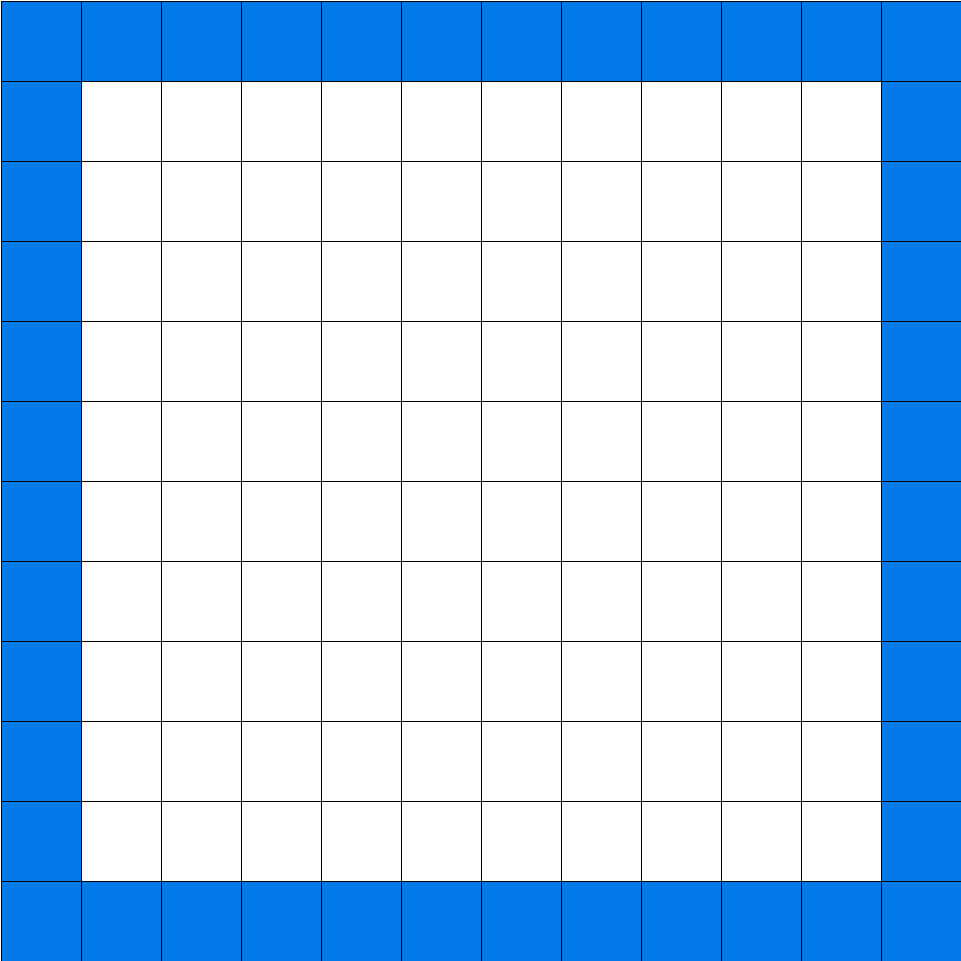
\includegraphics[scale=0.15]{figures/globaldomain.png}}
  \caption{\label{fig:globaldom}Domaine complet}
  \end{subfigure}%
  ~
  \begin{subfigure}[b]{0.5\textwidth}
    \centering
    \only<2>{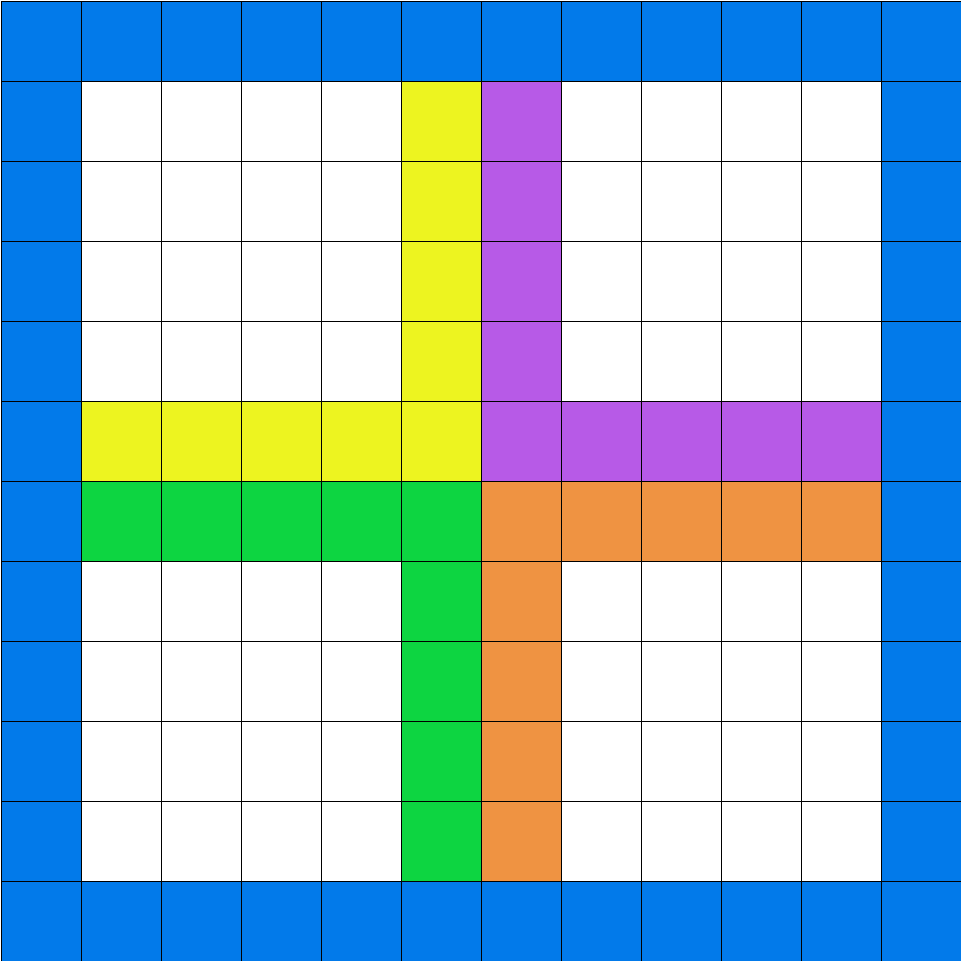
\includegraphics[scale=0.15]{figures/partitionnedomain.png}}
  \caption{\label{fig:partdom}Domaine partitionné}
  \end{subfigure}
  \caption{\label{fig:dom}Partitionnement du domaine}
\end{figure}
\end{frame}


\begin{frame}
  Problème numérique

\footnotesize
$$3\left( \frac{\partial u}{\partial x}\right) _{i-1} + 9\left( \frac{\partial u}{\partial x}\right) _{i} + 3\left( \frac{\partial u}{\partial x}\right) _{i+1} = \frac{1}{h}\left(  \frac{1}{4} \left( u_{i+2}-u_{i-2} \right) + 7 \left( u_{i+1} - u_{i-1} \right) \right) $$

\end{frame}


\begin{frame}
  Méthode Schwarz:
  \begin{itemize}
  \item Couplage inter-domaine elevé
  \item $\nearrow$ communications
  \item $\searrow$ taille des communications
  \end{itemize}
  Problème local modifié:
  \begin{itemize}
  \item Couplage inter-domaine faible
  \item $\searrow$ communications
  \item $\nearrow$ taille des communications
  \end{itemize}
\end{frame}


\subsection{Communications}
\begin{frame}
  \begin{figure}[!ht]
  \centering
  \begin{subfigure}[b]{0.5\textwidth}
    \centering
    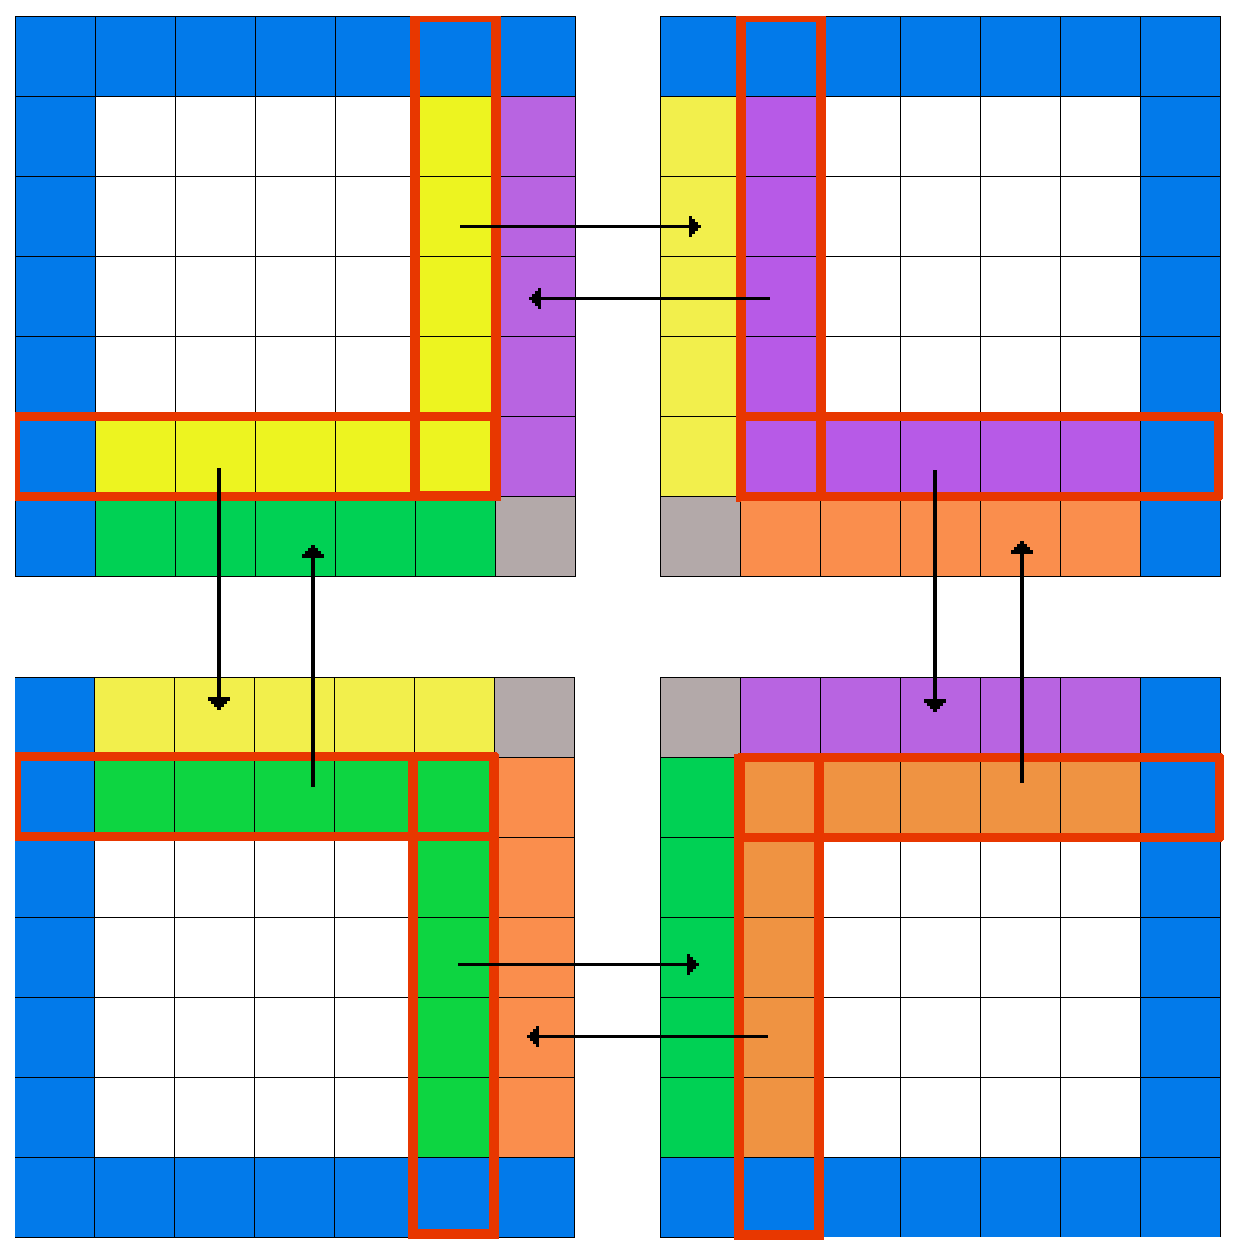
\includegraphics[scale=0.12]{figures/neigh1.png}
    \caption{\label{fig:comm_neigh}Echanges des zones de recouvrement}
  \end{subfigure}%
  ~
  \begin{subfigure}[b]{0.5\textwidth}
    \centering
    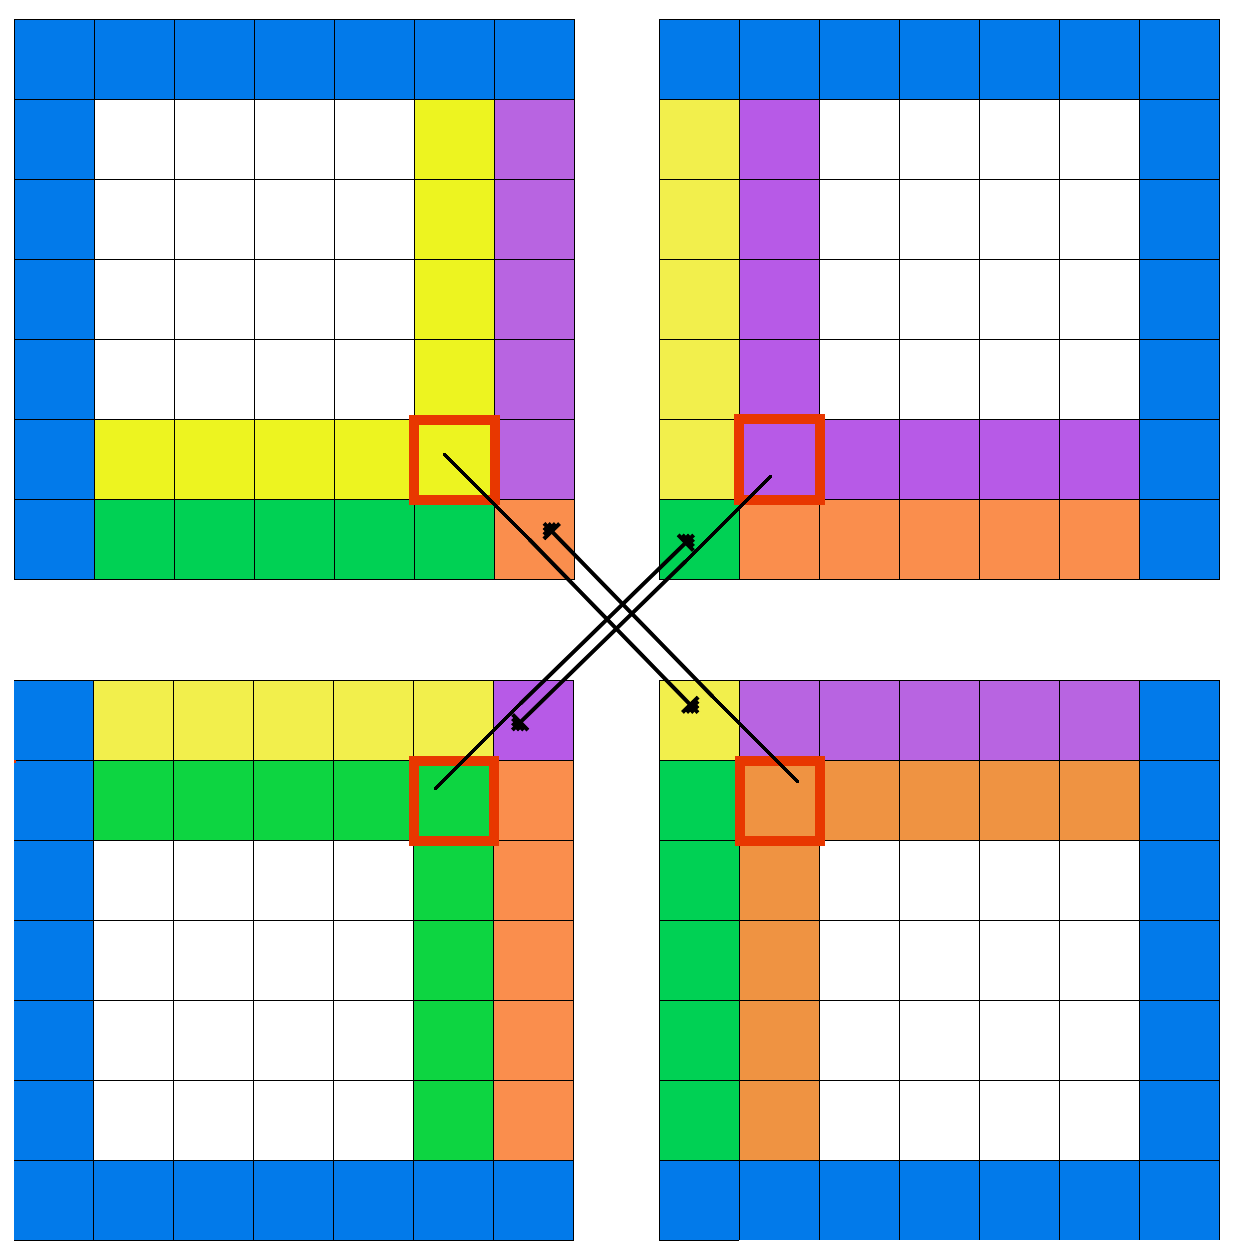
\includegraphics[scale=0.12]{figures/comm3.png}
    \caption{\label{fig:comm_diag}Echanges des coins}
  \end{subfigure}
  \caption{\label{fig:comm_neighbors}Echanges des zones de recouvrement avec MPI\_Neighbor\_alltoallv}
\end{figure}
  
\end{frame}

\begin{frame}
  \begin{figure}[!ht]
  \centering
  \begin{subfigure}[b]{0.5\textwidth}
    \centering
    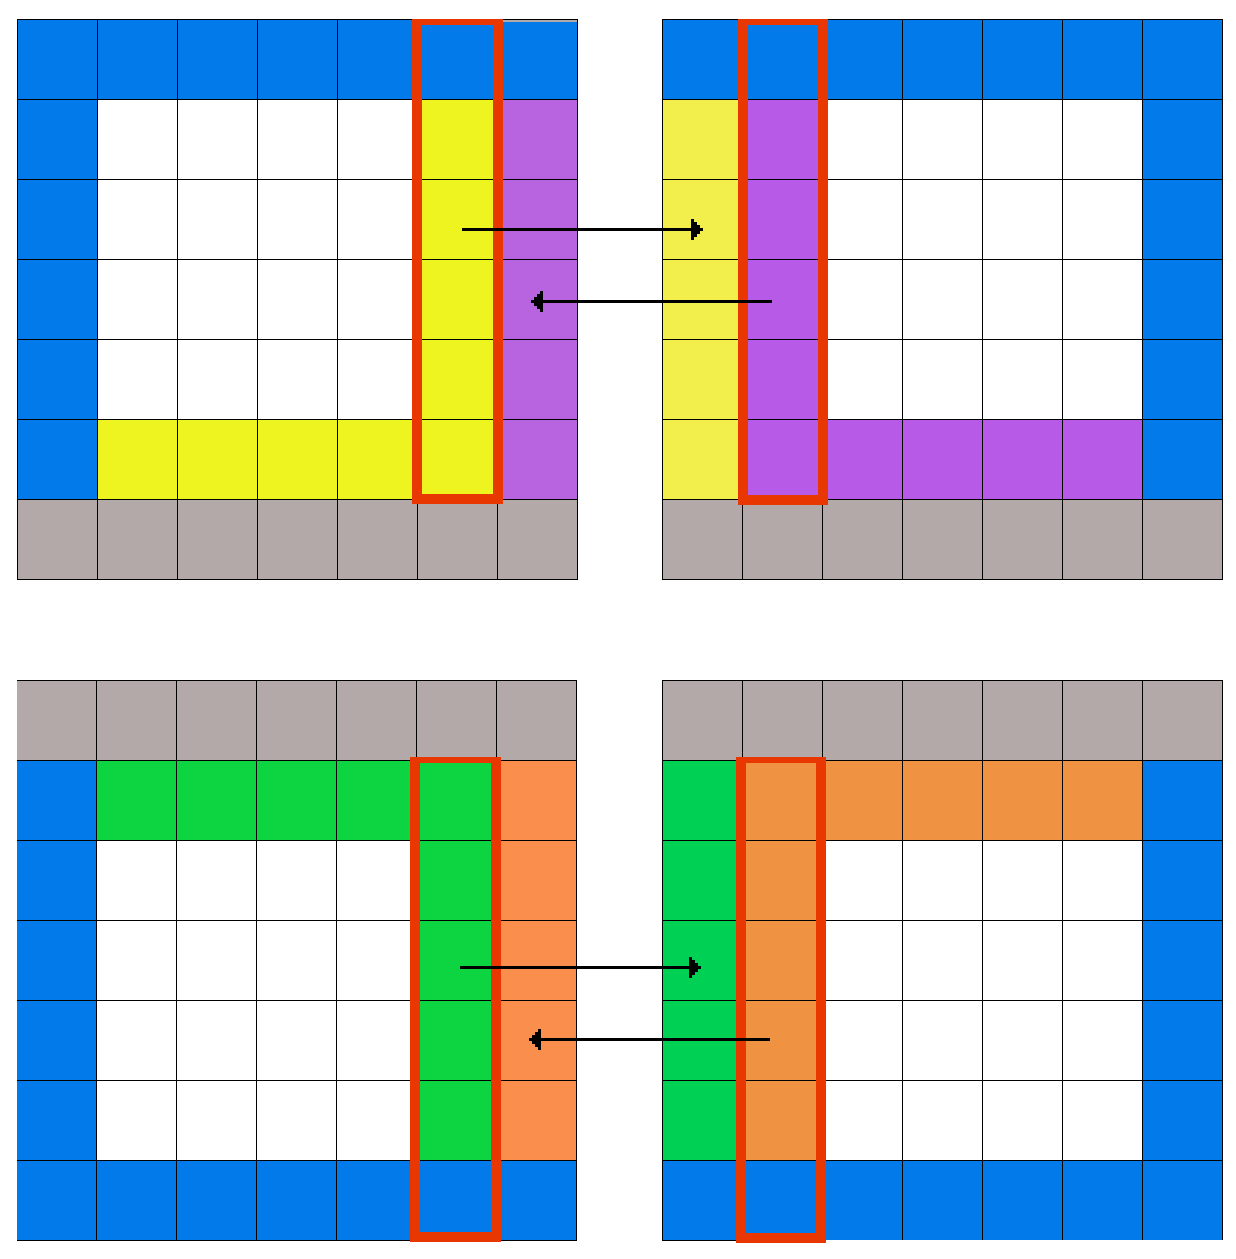
\includegraphics[scale=0.12]{figures/comm1.png}
    \caption{\label{fig:comm1}Echanges sur la dimension $x$}
  \end{subfigure}%
  ~
  \begin{subfigure}[b]{0.5\textwidth}
    \centering
    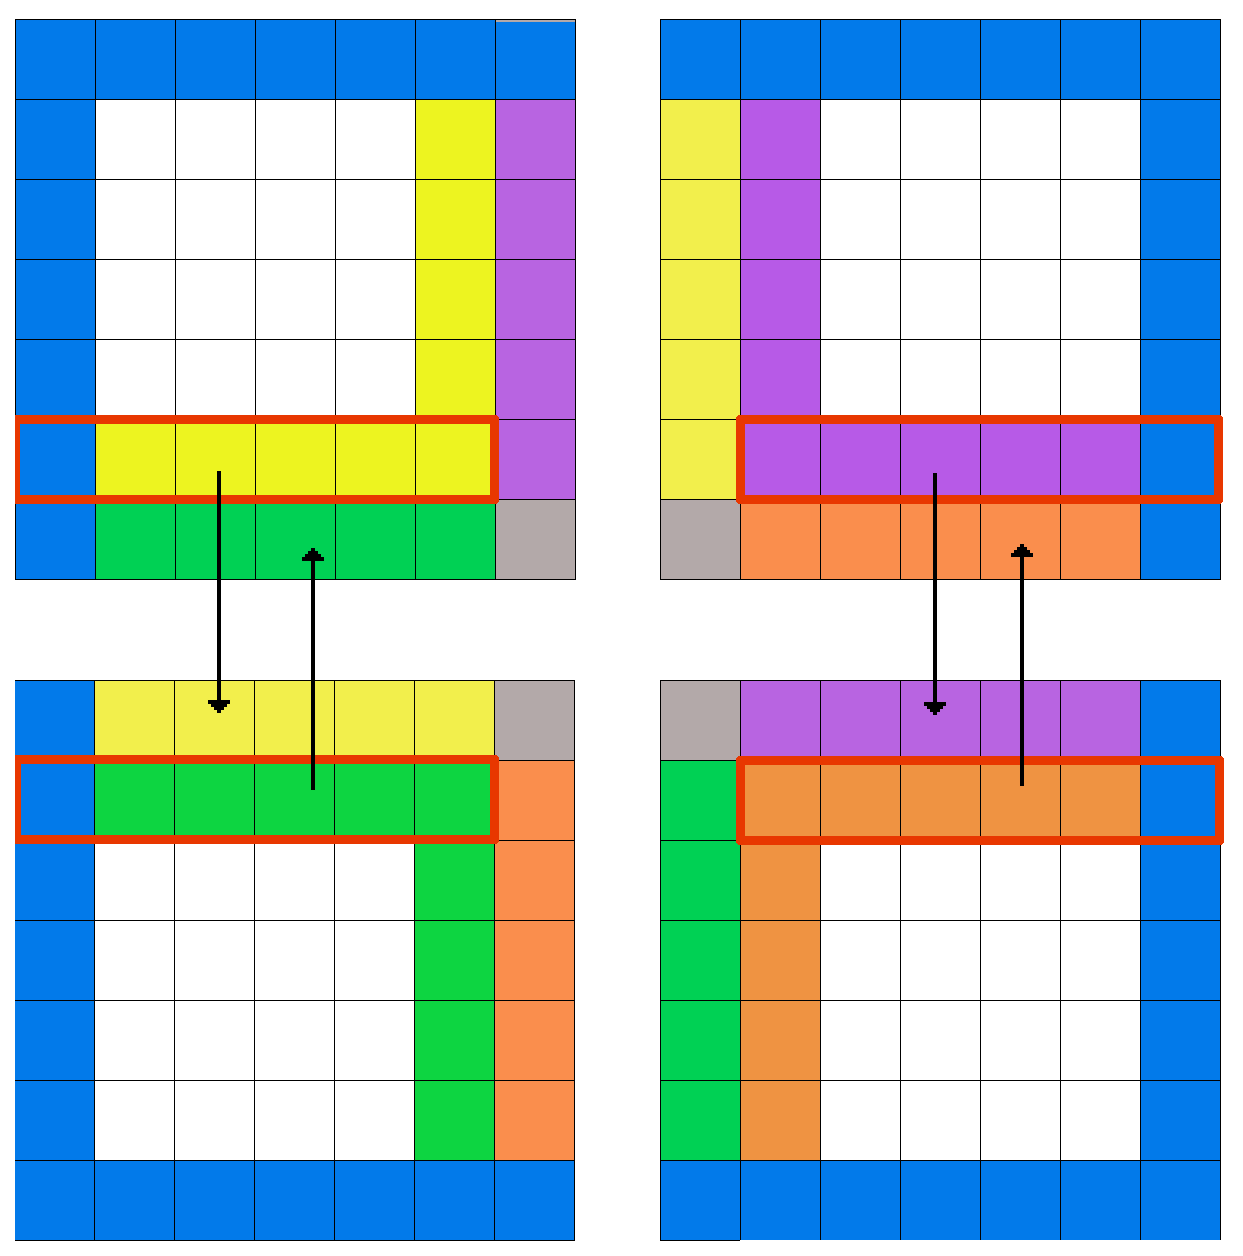
\includegraphics[scale=0.12]{figures/comm2.png}
    \caption{\label{fig:comm2}Echanges sur la dimension $y$}
  \end{subfigure}
  \caption{\label{fig:comm_synch}Echange des zones de recouvrement avec des communications non-bloquantes}
\end{figure}
\end{frame}


%
% Performances
%

\section{Etude des performances}
\subsection{Scalabilité forte}
\begin{frame}
  \begin{figure}[ht]
    \centering
    \includegraphics[page=2,scale=0.8]{gnuplot/bench_strong_nemo.pdf}
    \caption{\label{fig:label} }
  \end{figure}

\end{frame}


\subsection{Scalabilité faible}
\begin{frame}
  
\end{frame}

%
% Conclusion
%

\begin{frame}
  
\end{frame}

\end{document}
